\chapter{A quantum network of clocks}
\label{ch:Komar2014}
%From \cite{Komar2014}
%%%%%%%%%%%%%%%%%%%%%%%%%%%%%%%%%%%%%%%%%%%%%%%%

\section{Introduction}

The development of precise atomic clocks 
% has led to many scientific and
% technological advances that 
plays an  increasingly important role in  modern
society. Shared timing information constitutes a key resource for  
% positioning and 
navigation with a direct correspondence between timing accuracy and
precision in applications such as the Global Positioning System (GPS).
By combining  precision metrology and quantum networks, we propose 
% here 
a
quantum, cooperative protocol for operating a network of
geographically remote optical atomic clocks. Using non-local entangled states,
we demonstrate an optimal utilization of 
% the 
global 
% network 
resources, and show
that such a network can be operated near the fundamental precision limit set by
quantum theory.
Furthermore, the internal structure of the network, combined with 
% basic
quantum communication techniques, guarantees security both from internal
and external threats. Realization of such a global quantum network of clocks may
allow construction of a real-time single international time scale (world clock)
with unprecedented stability and accuracy.

 
With the advances of highly phase coherent lasers, optical atomic clocks
containing multiple atoms have demonstrated stability that reaches the standard
quantum limit (SQL) set by the available atom number 
% within a clock 
and interrogation time
\cite{Bloom2013, Hinkley2013, Nicholson2012}.
Reaching beyond the SQL, we stand to gain a significant improvement of clock
performance by preparing atoms in quantum correlated states (e.g., spin squeezed
states \cite{Leroux2010, Buzek1999}). Here we describe a new
approach to maximize the performance of a network composed of multiple clocks allowing one to gain the
advantage of all resources available at each node.
Several recent advances in precision metrology and quantum science,
along with future improvements in quantum control,  
may put this
approach within reach.  On the
 one hand, 
%  capabilities to maintain 
 phase coherent
optical links spanning the entire visible spectrum 
% and over macroscopic distances 
have been demonstrated, with the capability of delivering the most
stable optical oscillator from one color or location to another \cite{Ye2003,
Droste2013}.
On the other hand, quantum communication and entanglement techniques are
enabling distant quantum objects to be connected in a quantum network
\cite{cirac, kimble, acin}.
% , that can enable novel,
% extraordinary capabilities.
Combining these two technological frontiers, we show here that  a distributed
network composed of quantum-limited clocks separated by large distances -- as
appropriate, e.g., for satellite-based clocks possibly operated by different
nations -- can be operated  as an ultimate ``world clock'', where all members
combine their individual resources in a quantum coherent way  to achieve greater
clock stability and distribute this international time scale in real time for
all. 

The distributed architecture allows each participant of the network to profit
from a stability of the local clock signal that is enhanced by a factor
proportional to the total number of parties (as compared to an independent
operation of the individual clocks) without losing sovereignty or compromising
security. This cooperative gain strongly incentivizes joining the collaborative
network while retaining robustness against
 disruptions of communication channels.
%  by allowing the parties to fall back to
%  individual clock operation.
% Our scheme can be superior to an alternative approach of disseminating the time
% signal from a single location containing all qubits. 
On the one hand,
the local clocks can be used to identify and correct systematic errors
originating from the phase links. On the other hand, the nodes can fall
back to relying on the locally stabilized clocks if the phase links fail.
% since errors arising from imperfect phase links can be largely reduced by
% relying on the stabilized and locally available local oscillators.
% Our scheme is superior to an alternative approach of disseminating the time
% signal from a single location containing all qubits since, for short times,
% unavoidable fluctuations of the required phase stabilized links cancel the
% quantum gain. 
We demonstrate that by preparing quantum-correlated states of
remote clocks, the network can yield the best possible clock signal allowed by
quantum theory for the combined resources.
Furthermore, enabled through the use of quantum communication techniques,  such
a network can be made secure, such that only parties contributing to its
operation may enjoy the benefit of an ultra-precise clock signal. Besides
serving as a real-time clock for the international time scale,  the proposed
quantum network also represents a large-scale quantum sensor that can be used to
probe the fundamental laws of physics, including relativity and connections between space-time and quantum physics.

  










\section{The concept of quantum clock network}
\label{sec:QCN}

\reffig{fig:1} illustrates the basic concept for the proposed quantum
clock network.
We consider a set of $K$ atomic clocks (constituting the nodes of the network), each based on a large number of atoms (clock
qubits) serving as the frequency reference $\omega_0$ at different geographical
locations. In our approach,  each clock has its own independently operated local
oscillator (LO), $\mathcal{E}_j(t)\propto e^{i\nu_j t}$, with detuning $\delta_j
= \nu_j - \omega_0$, $(j=1,2\dots K)$. It keeps the time by interrogating its
qubits periodically, and uses the measurement data to stabilize the LO frequency
at the reference frequency of the atomic transition. However, as opposed to the
conventional approach, 
% in which each LO interrogates its own independent qubits,
we consider the situation in which each network node  allocates some of its
qubits to form entangled states stretching across all nodes. When interrogated
within a properly designed measurement scheme, such entangled network states
provide ultra-precise information about the deviation of the center-of-mass
(COM) frequency $\nu_\textrm{COM} = \sum_j \nu_j/K$ of all local oscillators
from the atomic resonance.  
\begin{figure}
\centering
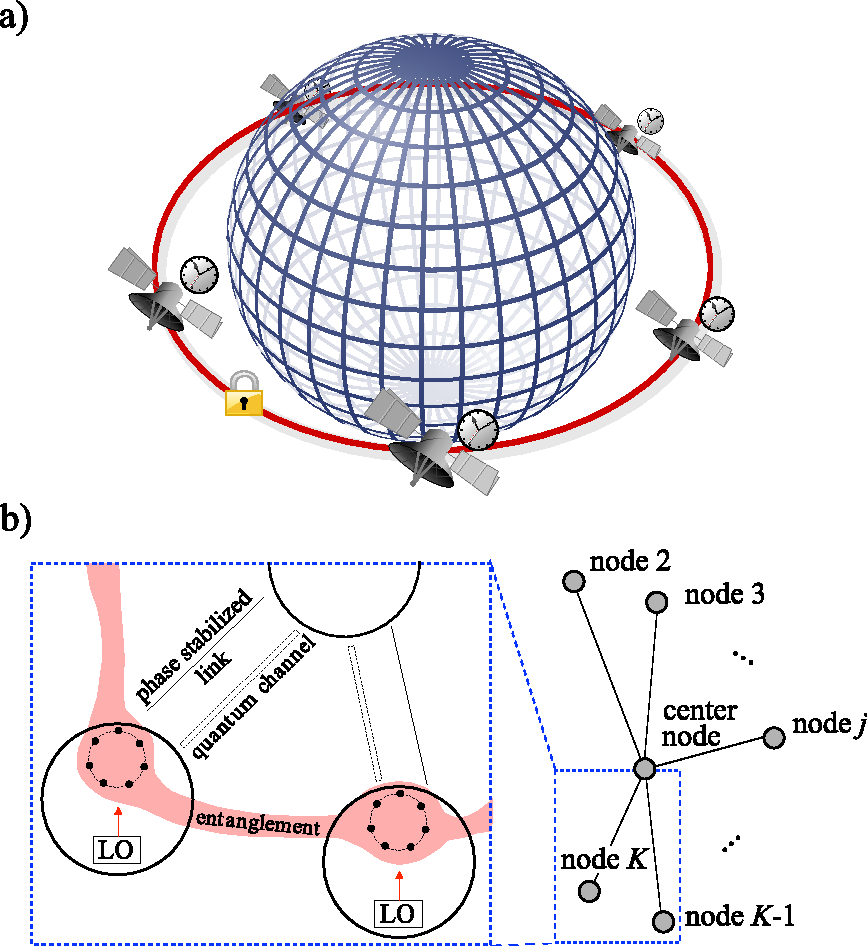
\includegraphics[width=0.8\textwidth]{./figs_Komar2014/fig1.pdf}
\caption
[The concept of world-wide quantum clock network]
{
\label{fig:1} The concept of world-wide quantum clock network.
a) Illustration of a cooperative clock operation protocol in which individual parties (e.g., satellite based atomic clocks from different countries) jointly allocate
their respective resources in a global network involving entangled quantum states. This guarantees an
optimal use of the global resources, achieving an ultra-precise clock signal
limited only by the fundamental bounds of quantum metrology and,
in addition, guaranteeing secure distribution of the clock signal.
 b) In addition to locally operating the individual clocks, the different nodes
 (i.e., satellites) employ network-wide entangled states to interrogate their
 respective local oscillators (LOs). The acquired information is sent to a particular node serving as
 a center where it is used to stabilize a center of mass mode of the different
 LOs. This yields an ultra-precise clock signal accessible to all network
 members.}
\end{figure}




% In the following, we describe the general working
% principle of  the proposed quantum clock network.



Each clock cycle consists of three stages: preparation of the clock atom state
(initialization), interrogation by the LOs (measurement) and correction of the
laser frequency according to the measurement outcome (feedback).
In the further analysis, we assume, for convenience, that in each interrogation
cycle one of the nodes plays the role of the center, which initiates
each Ramsey cycle and collects the measurement data from the other nodes via
classical channels [\reffig{fig:1}~b)], as well as LO signals via optical links,
 to feedback the COM signal.
(The role of the center can alternate to provide extra security, see
 Appendix \ref{app:Komar2014}). This information, in turn, can be utilized in a
 feedback cycle to yield a Heisenberg-limited stability of the COM clock signal
 generated by the network, which is
subsequently distributed to the individual nodes in a secure fashion.  As a
result, after a few cycles, the LOs corresponding to each individual node
achieve an accuracy and stability effectively resulting from interrogating atoms
in the entire network.



\section{Preparation of network-wide entangled states}
\label{sec:NWES}

In the initialization stage of each clock cycle, entangled states spanning
across the nodes at different geographical positions of the network are
prepared. In the following, we describe exemplarily how a single network-wide
GHZ state can be prepared. 
The entangled states employed in the proposed quantum network protocol -- which
is described in the following section -- consist of products of GHZ states of
different sizes. They can be prepared by repetition of the protocol that
we now describe.

For simplicity, we assume that each node $j$ ($j=1,\dots K$) contains an
identical number $n$ of clock qubits which we label as $1_j, 2_j,\dots n_j$ (in
Appendix \ref{app:Komar2014}, we discuss the case where the nodes contain
different amounts of clock qubits).
Further, we assume, for convenience, that the center node ($j=1$) has access to
additional $2(K-1)$ ancilla qubits $a_2,\dots, a_K,b_2,\dots,b_K$ besides the
$n$ clock atoms (a slightly more complicated procedure allows to refrain from
the use of ancilla qubits, see Appendix \ref{app:Komar2014}).
The entangling procedure starts at the center with the creation of a fully
entangled state of one half of the ancilla qubits $\{b_j\}$, and its first clock
qubit $1_1$. 
This can be realized, e.g.  with a single qubit $\pi/2$-rotation
(on qubit $1_1$)
and a collective entangling operation, which is equivalent to a series of
CNOT gates \cite{Nielsen_Chuang} (between $1_1$ and each $b_j$).
The result is a GHZ state, $[\ket{00\dots 0}_{1_1,b_2,b_3,\dots b_K} +
i\ket{11\dots 1}_{1_1,b_2,b_3,\dots b_K}]/\sqrt{2}$.
%performed with the local oscillator field at the center, $\mathcal{E}_1$. 
% \bel
% 	\ket{00\dots 0}_{c_1,c_2\dots c_K} \quad\rightarrow\quad \frac{\ket{0}_1 +
% 	i\ket{1}_1}{\sqrt{2}} \ket{0\dots 0}_{2\dots M} \quad\rightarrow\quad
% 	\frac{\ket{00\dots 0}_{1,2\dots M} + i\ket{11\dots 1}_{1,2\dots M}}{\sqrt{2}},
% \eel
In parallel, the center uses the other half of the ancillas $\{a_j\}$ to create single EPR pairs with each node $j\neq1$,
either by directly sending flying qubits and converting them to stationary
qubits, or by using quantum repeater techniques to prepare high-fidelity entanglement \cite{duan3}. As a result of this procedure, 
one part of the pair is stored at the center node (qubit $a_j$), while the other one
is stored at the $j$th  node (qubit $1_j$), forming the states $[\ket{00}_{a_j,1_j} +
\ket{11}_{a_j,1_j}]/\sqrt{2}$ for every $j$ (see \reffig{fig:entangling}).
\begin{figure}
\centering
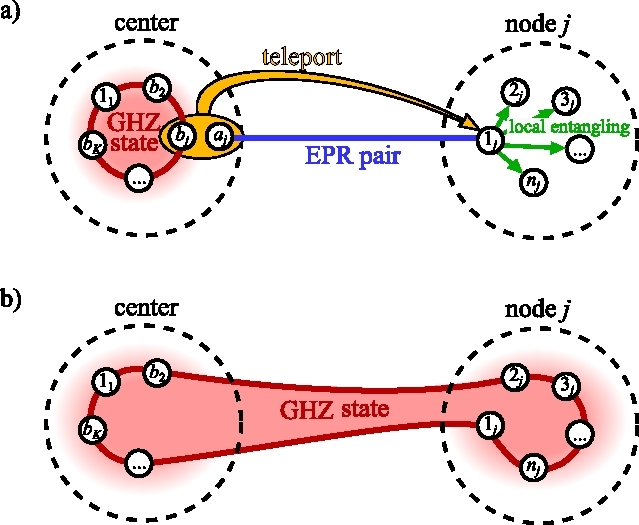
\includegraphics[width=0.7\textwidth]{./figs_Komar2014/fig2.pdf}
\caption
[Entangled state preparation between distant nodes]
{
\label{fig:entangling}
Entangled state preparation between distant nodes.
a) The center node $(j=1)$ initiates the initialization sequence by preparing a
local GHZ state across the qubits $\{b_j\}_{j=2}^K$ and $1_1$, as well as $(K-1)$ EPR pairs on
the qubit pairs $\{(a_j,1_j)\}_{j=2}^K$.
Quantum teleportation expands this GHZ state to the first qubit within each of
the individual nodes.
b) Originating from the teleported qubits, the nodes grow the GHZ state to
involve all the desired local qubits by employing local entangling
operations.
The procedure results in a common GHZ states over all atoms of the nodes.
 }
\end{figure}


%\subsection{Entangling}
% based on the existence of a secure central
% station,
Next, the center performs $K-1$ separate Bell measurements on
 its ancilla qubit pairs $\{(b_j, a_j)\}$. This teleports the state of qubit $b_j$ to
 qubit $1_j$
($j=2,\dots K$), up to a local single-qubit rotation, which is performed
after the measurement outcomes are sent to the node via classical channels.
The result of the  teleportations is a collective GHZ state
$\frac{1}{\sqrt{2}}\ket{00\dots 0}_{1_1,1_2,\dots 1_K} + i \ket{11\dots
1}_{1_1,1_2,\dots 1_K}$, stretching across the first qubits of all $K$ nodes.

In the final step of entangling, all nodes (including the center) extend the
entanglement to all of their remaining clock qubits. To do this, each node $j$
performs the collective entangling operation mentioned before based on
$1_j$ and targeting qubits $2_j, 3_j, \dots n_j$.  At the end of the protocol the different nodes share a common
GHZ state $[\ket{\mathbf{0}} + i\ket{\mathbf{1}}]/\sqrt{2}$, where
$\ket{\mathbf{0}}$ and $\ket{\mathbf{1}}$ are product states of all qubits
$\{i_j\;:\; i=1,2,\dots n,\; j=1,2,\dots K\}$ being in $\ket{0}$ or $\ket{1}$,
respectively. As discussed below, in practice the entanglement distribution can
be done  either via polarization- or frequency-entangled photons with frequency
difference in the microwave domain, in which case the ancillary qubits involved
in the entanglement distribution will be different from the clock qubits.
Typically, as part of the preparation process, time delays arise between the
initialization of different clock qubits. Its detrimental effects can be
entirely avoided by proper local timing or prior preparation of entanglement, as
discussed in Appendix \ref{app:Komar2014}.

\section{Interrogation}
\label{sec:SA}


The use of entangled resources 
% (in form of network-wide GHZ-like states) 
during
the interrogation phase enables an optimal use of the available resources via
the following procedure.  Assume we have a total of $\tilde N$ 
%($M$ being a positive integer)
qubits at
our disposal which are equally distributed between the $K$ nodes (indexed
$j=1,\hdots K$) and prepared in a non-local GHZ state $[\ket{\mathbf{0}} +
i\ket{\mathbf{1}}]/\sqrt{2}$, where $\ket{\mathbf{0 (1)}}\equiv\ket{0(1)}^{\otimes
\tilde N}$. During the
interrogation time $T$, a clock qubit at node $j$ picks up a relative phase $\phi_j = \delta_j
T$.
Due to the non-local character of the state, these phases accumulate in the total
state of the atoms  $[\ket{\mathbf{0}} + i e^{i\Phi}\ket{\mathbf{1}}]/\sqrt{2}$,
where the collective phase after the interrogation time $T$ is given as
\bel
\label{eq:1}
\Phi = \sum_{j=1}^K \frac{\tilde N}{K} \phi_j =
\tilde N \delta_\mathrm{COM} T,
\eel
where $\delta_\mathrm{COM} = \nu_\mathrm{COM} - \omega_0$.
% \bel
% 	\frac{1}{\sqrt{2}} \big(\ket{\mathbf{0}} + i
% 	e^{i\Phi}\ket{\mathbf{1}}),\qquad \Phi = \sum_{k=1}^M N_k \delta_k T .
% \eel
% This phase, $\Phi$, is sensitive to the weighted average of the detunings, ie.
% the center of mass of the detunings, $\nu_\mathrm{COM}-\omega_0 =
% \delta_\mathrm{COM} = [\sum N_k \delta_k] / [\sum N_k]$. By designing a
% measurement scheme estimating $\Phi$, we can get information on this COM
% detuning.
To extract the phase information picked up by the different GHZ states, 
% after each interrogation phase, 
the individual nodes $j$ measure their respective
qubits in the $x$-basis, and evaluate the parity of all measurement outcomes
$p_j = \pm 1$.
Subsequently, the nodes send this information to the center node via a classical
channel, where the total parity $p = \prod_{j} p_{j}$ is evaluated, and the
phase information is extracted \cite{Bollinger1996, Leibfried2004}. Note, that
only the full set $\{p_j |j=1\hdots K \}$ contains information. 
% This can be
% interpreted as only the center node holding the key,  namely its own measurement
% outcome $p_1$, to decode the phase information sent from the nodes.

The proportionality with $\tilde N$ in \refeq{eq:1} represents the quantum
enhancement in the estimation of $\delta_\mathrm{COM}$. However, for realistic
laser noise spectra, this suggested enhancement is corrupted  by the increase of
uncontrolled phase slips for a single GHZ
state 
%(i.e., undetectable transitions between fringes in a Ramsey
%experiment) 
\cite{Wineland1998}: Whenever, after the Ramsey time $T$, the phase $\Phi$ --
which due to the laser frequency fluctuations constitutes a random variable itself --
falls out of the interval $[-\pi,\pi]$ the estimation fails. This limitation
restricts the maximal Ramsey time to values $T < (\tilde
N\gamma_\mathrm{LO})^{-1}$, preventing any quantum gain in the estimation.


To circumvent this problem, we use entangled states consisting of products of
successively larger GHZ ensembles, see Appendix \ref{app:Komar2014} and 
\cite{Kessler2014}. In this approach, 
% interrogated network 
atoms are split into
several independent, shared groups.
% enables to correct for laser phase slips and 
%restores the quantum
%enhancement [REF:PRL paper]. 
% In the following, we apply these ideas to the clock network
% described above.
We write the number of the first group of atoms as $\tilde N =2^{M-1} K$, for
some natural number $M$.
Furthermore, the network shares additional groups of atoms, each containing
$2^{j} K$ ($j=0, \hdots M-2$) equally distributed between the nodes and prepared
in GHZ states. 
% \pk{The state of all the qubits can be written as
% $\left(\prod_{j=0}^{M-1} [\ket{0}^{2^jK} +
% i\ket{1}^{2^jK}]/\sqrt{2}\right)^{n_0}$, where $n_0$ is a small integer.}
Additionally, each node has a small number of uncorrelated atoms interrogated by
the LOs. Using a protocol reminiscent of the phase estimation algorithm
\cite{Kessler2014,Nielsen_Chuang, Giedke2006}, measurement results from each
level $j$ allow to directly assess the bits $Z_j \in \{0,1\}$ of the binary
fraction representation of the laser phase $\Phi_\mathrm{LO}=\delta_\mathrm{COM} T
=2\pi [(Z_1-1) 2^{-1} + Z_2 2^{-2} + Z_3 2^{-3} \hdots]$.
(See Appendix \ref{app:Komar2014} for details.)
This
% accounts for all phase slips {\it what does this mean?? up to the uncorrelated
% ensemble}, and
yields an estimate of $\Phi_\mathrm{LO}$ with Heisenberg-limited accuracy, up to a
logarithmic correction, see Appendix \ref{app:Komar2014}:
\bel 
	\Delta \Phi_\mathrm{LO} =\frac{8}{\pi}\log(N)/N,
	\label{eq2}
\eel 
even for Ramsey times beyond the limits of the laser frequency fluctuations [$T
> (\tilde N\gamma_\mathrm{LO}^{-1})$], where $N$ represent the total number of
clock atoms employed in the scheme. The logarithmic correction arises due to the
number of particles required to realize this (incoherent) version of the phase
estimation algorithm.

\section{Feedback}

The measured value of the phase  $\Phi_\mathrm{LO}$,
gives an estimate on the COM detuning
$\tilde\delta_\mathrm{COM}$ after each Ramsey cycle, which is subsequently used
by the center node to stabilize the COM laser signal.
To this end, the center generates the COM of the frequencies. Every node sends
its local oscillator field $\mathcal{E}_i$ to the center via phase-stable
optical links, and the center synthesizes the COM frequency $\nu_\mathrm{COM}$ by
averaging the $\nu_j$ frequencies with equal weights.
% \footnote{With different
% number of qubits at each node, the weighted average needs to be taken.}
This can be implemented via heterodyne beat of the local oscillator in the
center against each incoming laser signal, resulting in $K$ beat frequencies.
Synthesizing  these beat frequencies allows the
local oscillator of the central node to phase track $\nu_\mathrm{COM}$.
%Subsequently, the center uses the 
%acquired information about $\delta_\mathrm{COM}$ to stabilize $\nu_\mathrm{COM}$ by
%application of digital frequency shifts. 
The center distributes the stabilized clock signal to different members of the network by sending individual error
signals $\tilde \delta_j = \tilde \delta_\mathrm{COM} + (\nu_j - \nu_\mathrm{COM})$
to all nodes $j$, respectively, and corrects its own LO as well, accordingly.
Alternatively, the center can be operated to provide restricted feedback
information to the nodes, see Appendix \ref{app:Komar2014}.



\section{Stability analysis}
\label{sec:comp}

In this section, we demonstrate that the proposed quantum clock network achieves
the best clock signal, allowed by quantum theory for the available resources, i.e.
the total atom number. 
% Rather than individually operating their respective LOs the
% joint use of resources allows the network to  directly interrogate and stabilize
% the COM mode of the lasers. 
To quantify this cooperative gain, we compare
networks of different types (classical or quantum mechanical interrogation of
the respective LOs) and degrees of cooperation (no cooperation, classical, or
quantum cooperation).


First, we analyze the stability of the proposed quantum clock network,
corresponding to the case of quantum interrogation and cooperation (curve a in
\reffig{fig:comp}). In this case, the analysis resulting in \refeq{eq2}
suggests that near Heisenberg-limited  scaling with a total atom number can be achieved
for the entangled clock network. 
In particular, for a given total particle number $N$ and for averaging times
shorter than the timescale set by individual qubit noise $\tau < 1/(\gamma_i N)$
(where $\gamma_i$ is the atomic linewidth, the factor $N$ results from the
enhanced decoherence of the entangled interrogation state
\cite{Huelga1997}), the network operation achieves a Heisenberg-limited Allan
deviation (ADEV) of the COM laser mode
\begin{align}
\label{eq:ADEV1}
 	\sigma_y(\tau) 
%  	=  \frac{1}{\omega_0 \sqrt{n_0}2^{M}K} \frac{1}{\tau}
	\sim \frac{ \sqrt{\textrm{log}(N)}}{\omega_0 N} \frac{1}{\tau},
\end{align}
up to small numerical corrections (see Appendix \ref{app:Komar2014}).
% Here, the number of GHZ copies per group $n_0\sim \textrm{log}(N)$ ($N\approx n_0
% 2^{M+1} K $) is found after optimization, and
% gives rise to a logarithmic correction in the total particle number.
The $1/\tau$ scaling results from the effective cancellation of the low
frequency part of the laser noise spectrum, achieved
by the cascaded protocol described above, possibly in combination with additional stages of uncorrelated interrogations using varying Ramsey times \cite{Rosenband2013,Borregaard2013}, see \cite{Kessler2014}.
This allows the cycle time $T$ (which is assumed to be equal to
the interrogation time) to be extended to the total available measurement time
$\tau$.
\begin{figure}
\centering
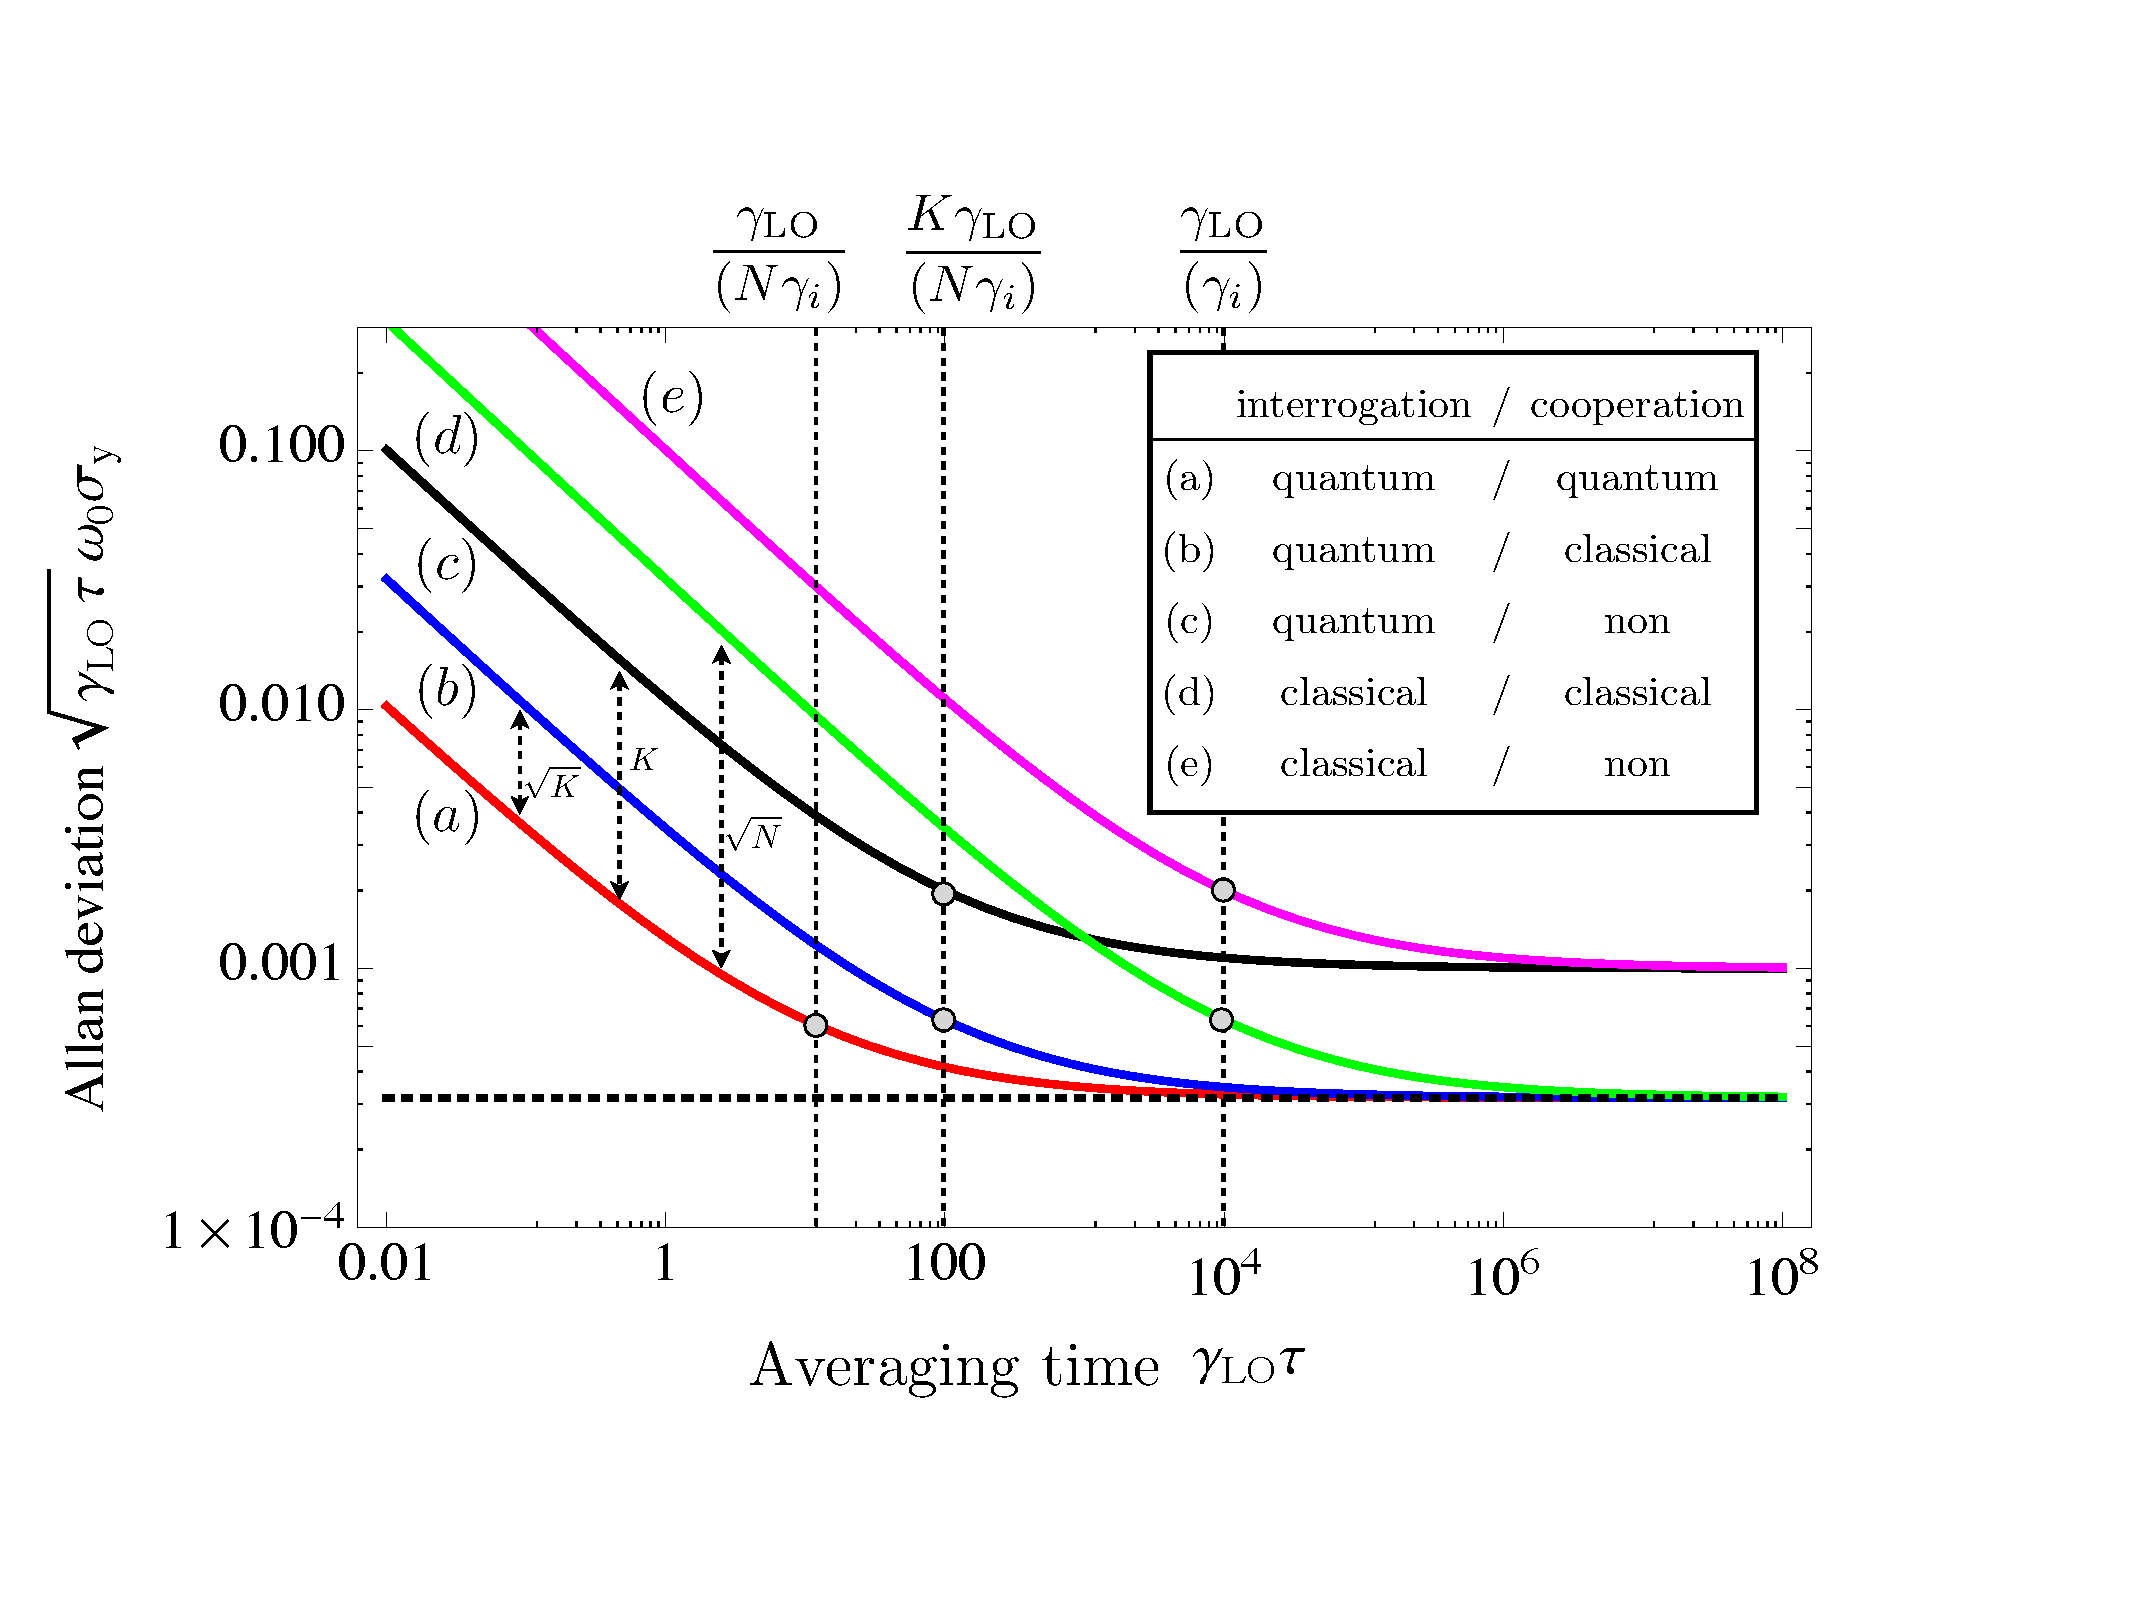
\includegraphics[width=1\textwidth]{./figs_Komar2014/fig3.pdf}
\caption
[Performance of different operation schemes]
{
\label{fig:comp}
Performance of different operation schemes. Comparison of
the achievable (rescaled) Allan deviation $\sqrt{\gamma_\mathrm{LO} \tau} \omega_0 \sigma_y$ using clock networks of different types and degrees of
cooperation. (a) the proposed protocol realizing quantum interrogation and
cooperation, (b) quantum interrogation and classical cooperation, (c) quantum
interrogation and no cooperation, (d) classical interrogation and classical
cooperation, (e) classical interrogation and no cooperation (cf. text). The
dotted base line represents the fundamental bound arising from the finite width
of the clock atoms transition
[compare \refeq{eq:ADEV2}]. This optimal stability can be attained only via cooperation between the
nodes.
The quantum clock network (a) represents the optimal form of cooperation, and reaches this boundary faster than any other
operational mode. Parameters are $N=1000$, $K=10$,
$\gamma_i=10^{-4}\gamma_\mathrm{LO}$.
 }
\end{figure}



Eventually, for large averaging times $\tau > 1/(\gamma_i N)$ the
Ramsey time becomes fundamentally limited by individual
noise processes that determine the atomic linewidth $T\leq 1/(\gamma_i N)$.
As a result, the $1/N$ scaling breaks down, and the ADEV returns to the square
root scaling with both the employed particle number and averaging time,
\begin{align}
\label{eq:ADEV2}
	\sigma_y(\tau) \sim \frac{ 1}{\omega_0 \sqrt N}
	\sqrt{\frac{\gamma_i}{\tau}},
\end{align}
up to constant numerical factors.  \refeq{eq:ADEV2} results from fundamental
quantum metrological bounds \cite{Escher:2011fn} (In the case of
dominating trap losses, the loss rate simply replaces $\gamma_i$ in the above
formula.), and represents the best conceivable clock stability in the presence
of individual particle decoherence which, in a network, can only be achieved via cooperation. Independently operating a clock, in contrast, can only achieve a stability scaling with the local number of atoms, i.e. $\sigma_y(\tau)\propto \sqrt{K/N}$.


 \reffig{fig:comp} illustrates the comparison of entangled clock network with
other approaches.
A network in which the $K$ nodes cooperate classically (curve b in
Fig.~\ref{fig:comp}), by locally measuring the individual phase deviation
$\phi_j$, and combining the outcomes via classical channels, outperforms
individually operated clocks (curve c) by a factor of $\sqrt K$ 
(for both cases, assuming optimal
quantum interrogation for individual nodes
\cite{Kessler2014,Borregaard2013_nearHeisenberg}).
The quantum network protocol (curve a)
increases this cooperative advantage by an additional factor of $\sqrt K$ for
short averaging times, reaching Heisenberg-limit, Furthermore the ADEV
converges to the fundamental bound [\refeq{eq:ADEV2}] $K$ times faster compared
to the case of classical cooperation (curve b).
Although an optimal, classical, local protocol
(e.g. \cite{Rosenband2013, Borregaard2013}), combined with classical
cooperation (curve d), eventually reaches the same
bound [\refeq{eq:ADEV2}],
% in this case, the obtainable stability is always
 % limited by the standard quantum limit with regard to the
% employed resources, $\sigma_y(\tau) \propto 1/\sqrt N$. Therefore,
this approach is atom-shot noise limited, and hence its stability is reduced by
a factor of  $\sqrt N$ for short averaging times [compare \refeq{eq:ADEV1}]
compared to the quantum network protocol.  Hence, the optimal stability
[\refeq{eq:ADEV2}] is reached at averaging times that are $N$ times longer
than for the proposed quantum network. Naturally, all of the above approaches
are superior to a classical scheme without cooperation (curve e).

As a specific example, we first consider ion clocks that can currently achieve a
stability of $2.8\times 10^{-15}$ after $1~\mathrm{s}$ of averaging time
\cite{Chou2010}. The entangled states of up to 14 ions has already been
demonstrated \cite{Monz2011} as was the entanglement of remote ions
\cite{Maunz2007}. We consider a network of ten clocks, each containing ten ions.
Using $\mathrm{Al}^+$ ($\omega_0 = 2\pi \times 1121~\mathrm{THz}$, $\gamma_i = 2\pi
\times 8~\mathrm{mHz}$), we find that the quantum cooperative protocol can reach
$4\times 10^{-17}$ fractional frequency uncertainty after $1~\mathrm{s}$. Larger
improvements could potentially be achieved using e.g. $\mathrm{Yb}^+$ ions, due to the long coherence time ($2.2\times
10^4~\mathrm{s}$) of its octupole clock transition.

The quantum gain could be even more pronounced for neutral atomic clocks. For a
network consisting of ten clocks similar to the one operated in JILA
\cite{Bloom2013}, each containing 1000 neutral atoms with central frequency
$\omega_0 = 2\pi\times 429~\mathrm{THz}$ and linewidth $\gamma_i = 2\pi \times
1~\mathrm{mHz}$,  the quantum cooperative scheme can achieve a stability of $\sim
2\times 10^{-18}$ after 1s averaging, and is an order of magnitude
better than the best classical cooperative scheme.  Future advances,
employing clock transitions with linewidths of a few tens of
$\mu\mathrm{Hz}$ (such as erbium), could possibly allow for further
improvement, achieving fractional frequency uncertainty beyond $10^{-20}$
after $\tau \sim 100~\mathrm{s}$. This level of stability is in the same order of
magnitude as the required sensitivity to successfully use the network as a
gravitational interferometer \cite{Schiller2008}.


So far we have assumed perfect operation and infinitely fast entanglement
distribution rates. In Appendix \ref{app:Komar2014}, we analyze these assumption
and find that the advantage of our scheme persists provided that fidelity  of the local collective
entangling \cite{MSgate} (which creates a GHZ state of $N/K$ qubits) exceeds the
threshold fidelity $F_\mathrm{th}$, where $1-F_\mathrm{th} \sim 1/(K\log N)$, and
the EPR sharing rate is higher than $R_\mathrm{EPR}\sim (\log N)^2 \gamma_i$.
For the optical clock example presented above, $F_\mathrm{th} \sim 0.99$, and
$R_\mathrm{EPR} \sim 1~\mathrm{Hz}$. While local operations with fidelity
$\sim 0.95$ have been realized for $N\sim 5$ ions \cite{Monz2011}, the errors
in such operations increase with $N$, making this realization more challenging.




\section{Security}
\label{sec:Security}
A network with such precise time-keeping capabilities can be subject to both internal
and external attacks. Effectively countering them is crucial to establish a
reliable ground for cooperation. We consider the network secure if the
implemented countermeasures can prevent external parties from benefiting from
the network (eavesdropping), as well as effectively detect any malicious activities of any of the members (sabotage).

Sabotage describes the situation where one of the nodes -- intended or
unintended -- operates in a damaging manner. For example, one node
% that is blatant enough to not comply with the formal requirements of the
% protocol is easily detected by the center within the time period of a single
% cycle, and then the particular node gets excluded from further cycles. More
% stealthy types of sabotage
could try sending false LO frequencies or wrong measurement bits in the hope of
corrupting the collective measurement outcomes. In order to detect such
malicious participants, the central node can occasionally perform assessment
tests of the different nodes by teleporting an uncorrelated qubit state
$[\ket{0} + e^{i\chi}\ket{1}]/\sqrt{2}$, where $\chi$ is a
 randomly chosen phase known only to the center. By checking for statistical
discrepancies between the measurement results and the detuning of the LO signal
sent by the node under scrutiny, the center can rapidly and reliably determine
whether the particular node is operating properly (See \reffig{fig:security}a
and Appendix \ref{app:Komar2014}),
however this strategy breaks down, if multiple sabotage attacks
happen within a short time.
\begin{figure}
\centering
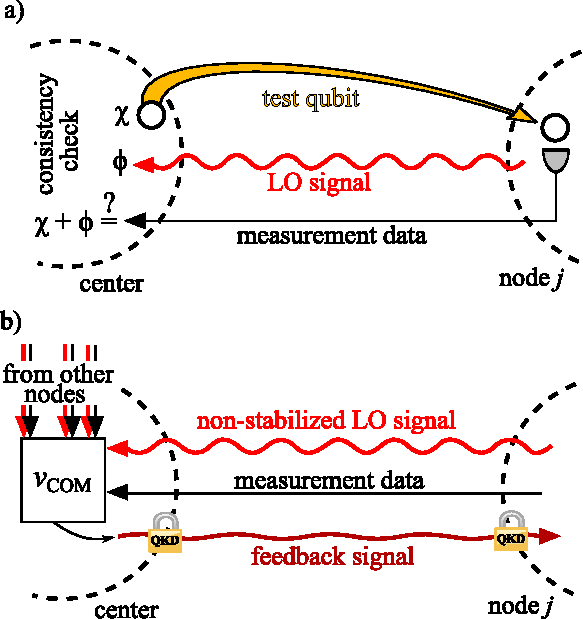
\includegraphics[width=0.7\textwidth]{./figs_Komar2014/fig4.pdf}
\caption
[Schematics of security countermeasures]
{
\label{fig:security}
Schematics of security countermeasures.
a) The center node can choose to test any node $j$ by teleporting a disentangled
qubit with a certain phase rotation. A properly operating node creates a local
GHZ state $[\ket{\mathbf{0}} + e^{i\chi}\ket{\mathbf{1}}]/\sqrt{2}$ from the
sent qubit,
 measures the parity of the GHZ state, and sends it to the center. The
measured parity holds information on the phase $\phi' = \chi + \phi$, where
$\phi$ is the accumulated phase of the LO at the node. The center verifies
$\phi$ by comparing it with the classically determined  phase of the sent LO
signal with respect to the COM signal.
b) Eavesdropping can be prevented by prescribing that only the non-stabilized LO
signals are sent through  classical channels and encoding the radio frequency
feedback signal with phase  modulation according to a shared secret key.
}
\end{figure}


Eavesdropping, i.e., the unauthorized attempt to access the stabilized
$\nu_\mathrm{COM}$ frequency, can be prevented by encoding the classical channels,
over which the center and the nodes exchange feedback signals, using quantum key
distribution protocols \cite{Gisin2002}. Our protocol can keep the stabilized
signal hidden from outsiders by mixing the feedback signal with the LO signal at each node only
after the non-stabilized LO has been sent to the center (see
\reffig{fig:security}b and Appendix \ref{app:Komar2014}). As a result, even if  all LO signals are intercepted, the eavesdropper is able to access
only the non-stabilized COM signal. Furthermore, the center exclusively can decode the
measurement results sent by the individual nodes using its own measurement outcomes as mentioned above. 
As a result, the stabilized COM signal remains
accessible exclusively to parties involved in the collaboration.

Finally, we note that a distributed operation offers significant security
advantages over an alternative approach of having all resources combined in one
place from where the signal is distributed. In case of a physical attack of the
network, disabling the center or the communication links, the nodes can fall
back to an independent clock operation using their local resources.

\section{Outlook}

One of the advantages of the proposed quantum clock network involves its ability
to maintain and synchronize the time standards across multiple parties in
real-time. 
% This can be achieved with classical cooperation schemes as well,
% however it arises naturally in the quantum scheme. 
Unlike the current world time standard, where the individual signals from
different clocks are averaged and communicated with a time delay (a so called
paper clock), in our quantum clock network, all participants have access to the
ultra-stable signal at any time.
This makes it possible to measure systematic errors of different clocks in
real time, which in turn allows to correct them \cite{Bloom2013}, unlike in the
case of the paper clock which has to rely on the retrospectively averaged time 
signals (see Appendix \ref{app:Komar2014}). 
The enhanced stability of the network signal hereby allows for longer Ramsey
times in the control measurements used to determine the systematics of the
single clock.
% The longer Ramsey time allows this measurement to be carried
% out with precision limited only by the accuracy of the network.
Furthermore, by having full access to their local clocks the different parties
keep  their full sovereignty and ensure security, as opposed to a joint
operation of a single clock.

Realization of the full-scale network of the type described here will require a
number of technological advances in both metrology and experimental quantum
information science. 
% Practical realization can be based on optical atomic 
% clocks involving either trapped ions \cite{Chou2010} or neutral atoms
% \cite{Nicholson2012}.
% While ions provide a more straightforward implementation of the preparation of entangled qubit states \cite{Cirac2000, Monz2011}, state of the art neutral atom clocks
% feature large atom number resulting in better stability and potentially more
% significant quantum enhancement \cite{Nicholson2012}.
The remote entanglement can be implemented by using recently demonstrated
techniques for individual atom-photon entanglement \cite{Olmschenk2009,
Chou2007, togan, Bernien2013, Riste2013}. Since the teleportation protocol
requires quantum links capable of sharing EPR pairs with sufficiently high
repetition rate and fidelity, entanglement purification \cite{Dur1999} and
quantum repeater techniques \cite{duan3} will likely be required. In
practice, qubits used for entanglement distribution may not be ideal for clocks.
 However, as noted previously  remote entanglement does not need to involve
coherent qubits at optical frequencies (e.g., polarization entanglement can be
used). In such a case,   the use of hybrid approaches, combining  different
systems for entanglement and local clock operations, may be warranted.
Similarly, signals from clocks employing different transition frequencies
can be coherently connected by frequency combs, allowing clocks with different
clock qubits to participate.
% So far we have considered schemes requiring individual qubit addressing, however
It might also be interesting to explore if high-fidelity entangled EPR pairs can
be used to create remote entangled states of spin-squeezed type \cite{Leroux2010,
Sherson2006, Ma2012}, or by following the proposed approach for cat state
preparation in atomic ensembles \cite{McConnell2013}, 
or using collective interactions (such as \cite{MSgate}) and repetitive teleportation 
\cite{Andersen2013}.
% Alternatively, recently demonstrated  individual addressing in optical lattices
% \cite{Bakr2009, Lee2013} could be combined with entanglement swapping techniques
% to directly entangle optical lattice clocks.
% Lastly, the use of a continuous variable approach can be potentially explored to
% create squeezed atomic states across the network \cite{Sherson2006, Ma2012}. The
% use of collective measurements may allow one to reach Heisenberg limited
% stability \cite{Borregaard2013_nearHeisenberg}, while  squeezing can be transferred
% from photons to atomic ensembles \cite{Sherson2006, Hammerer2010}. An important
% open question of sensitivity of these techniques to photon losses needs to be
% addressed. 
In addition, while space-based communication networks will be capable
of maintaining optical phase coherence for the links between clocks, we note
that establishing ground-space coherent optical links remains a technical
challenge and requires an intense research effort which has recently started
\cite{Djerroud2010}.
% Beyond specific implementations, a number of other research directions may be
% explored. These include optimal eavesdropping, error correction and security
% strategies, robust feedback approaches minimizing technical imperfections such
% as Dick effect \cite{Santarelli1998}, as well as novel applications taking
% advantage of enhanced clocks with short averaging time.
Finally, if the entire network is spanned by satellites in space, the on-board
local oscillators can further benefit from the much lower noise level compared
to ground-based clocks.

If realized, such a quantum network of clocks can have important scientific,
technological, and social consequences. Besides creating a world platform for
time and frequency metrology, such a network may find important applications to
a range of technological advances for earth science \cite{Tapley2005},
precise navigation of autonomous vehicles and space probes (requiring high
 refresh rate), and to the test and search for the fundamental laws of
nature, including relativity and the connection between quantum and
gravitational physics \cite{Abramovici1992, Seidel2007, Schiller2008, Wolf2008}.
In order to explore these exciting applications one can either use the excellent
common frequency reference generated by the clock network, or, alternatively,
prepare modified collective states of different nodes that can directly measure
the specific signal under study. 
 






